\chapter{FPGA\label{FPGA}}
As briefly mentioned in the introduction, FPGAs consist of an array of logic
gates. In this section we will give an overview on how such components work and
different ways of configuring them. Modern FPGAs may also include of other
components, such as processors and multipliers which is out of the scope of
the present thesis.

\section{Lookup tables}

\textit{Lookup tables} (LUT), are crucial component of FPGAs. We will first
introduce some preliminary information on \textit{boolean functions}.

\begin{definition}
    A boolean function is a function that is defined on two element sets, i.e.
    $\{0,\ 1\}$, $\{\text{true},\ \text{false}\}$, ..., etc.

    Without loss of generality we can define a boolean function $f$ to be a
    function of form

    \[f \colon \{0,\ 1\}^N \rightarrow \{0,\ 1\}, \quad \text{where $N$ is the
    size of the input}\]

    Any boolean function can be represented by \textit{truth table}. A truth
    table represents all the possible outputs when a function $f$ is evaluated.
    Consequently, the size of the truth table is $2^N$.
\end{definition}


\begin{example}
    \label{ex:boolean_function}

    Hereon the addition $+$ and multiplication $\cdot$ is understood as the
    usual boolean addition and multiplication.

    \[
    f \colon \{0,\ 1\}^3 \rightarrow \{0,\ 1\}, \quad (A, B, C) \mapsto A + B \cdot C
    \]

    There are $2^3 = 8$ possible values for the function $f$. Table
    \ref{tab:example_truth_table} represents the truth table. We'll look at how
    this could be represented using logic gates in a later section.
    \begin{table}[H]
        \centering
        \begin{tabular}{|l|l|l|l|}
            \hline
            A & B & C & Out \\ \hline
            0 & 0 & 0 & 0   \\ \hline
            0 & 0 & 1 & 1   \\ \hline
            0 & 1 & 0 & 0   \\ \hline
            0 & 1 & 1 & 1   \\ \hline
            1 & 0 & 0 & 0   \\ \hline
            1 & 0 & 1 & 1   \\ \hline
            1 & 1 & 0 & 1   \\ \hline
            1 & 1 & 1 & 1   \\ \hline
        \end{tabular}
        \caption{Truth table for function $f$}
        \label{tab:example_truth_table}
    \end{table}


    In fact these truth tables are what allows the re-configuration of FPGAs, by
    replacing the values in the truth tables we can make it evaluate a different
    function.
\end{example}

\begin{definition}

    A \textit{lookup table} is a truth table that is represented in continuous
    memory. LUTs are implemented are using $N:1$ \textit{multiplexers}. A
    multiplexer is a component that simply maps multiple inputs into a single
    output, the internals of it is out of the scope of this thesis. Using $N$-bits
    of memory to store all the answers of the truth table in memory we can evaluate
    any boolean function.

    In 1990 there was a study on how many inputs a LUT should have. If
    there were more inputs it would allow for more complex logic. Though adding more
    inputs would also make the chip slower, the generally accepted number is
    between three and four \citep{RoseArchitecture}.

\end{definition}

\subsection{Delay flip-flop}
LUTs alone are not enough to be able to be Turing complete as we cannot store
state. What we need is some way to store information, this is where the
\textit{delay(D) flip-flops} come in. A D flip-flop can store a single bit of
data, this is incredibly useful as it can be used to store state. In Figure
\ref{fig:lut_flipflop} we can see an example of a D flip-flop. Our input for
the flip-flop is D, our output is Q, and the triangle underneath D is the
clock. The D flip-flop works around the clock, it can only read the input
whenever the clock is on a \textit{rising edge}. A rising edge is when the
clock sends a signal to the flip-flop to tell it to check the data value. We
can an example of this in Figure \ref{fig:flipflop_func}. The output Q is only
changed to high after the second cycle and waits a cycle to go to low after the
third cycle.

\begin{figure}[H]
    \begin{subfigure}[b]{.4\textwidth}
        \centering
        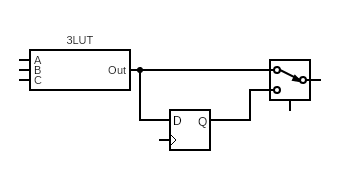
\includegraphics[scale=0.4]{lut_structure.png}
        \caption{An example of how a lookup table could be implemented}
        \label{fig:lut_flipflop}
    \end{subfigure}
    ~
    \centering
    \begin{subfigure}[b]{.4\textwidth}
        \centering
        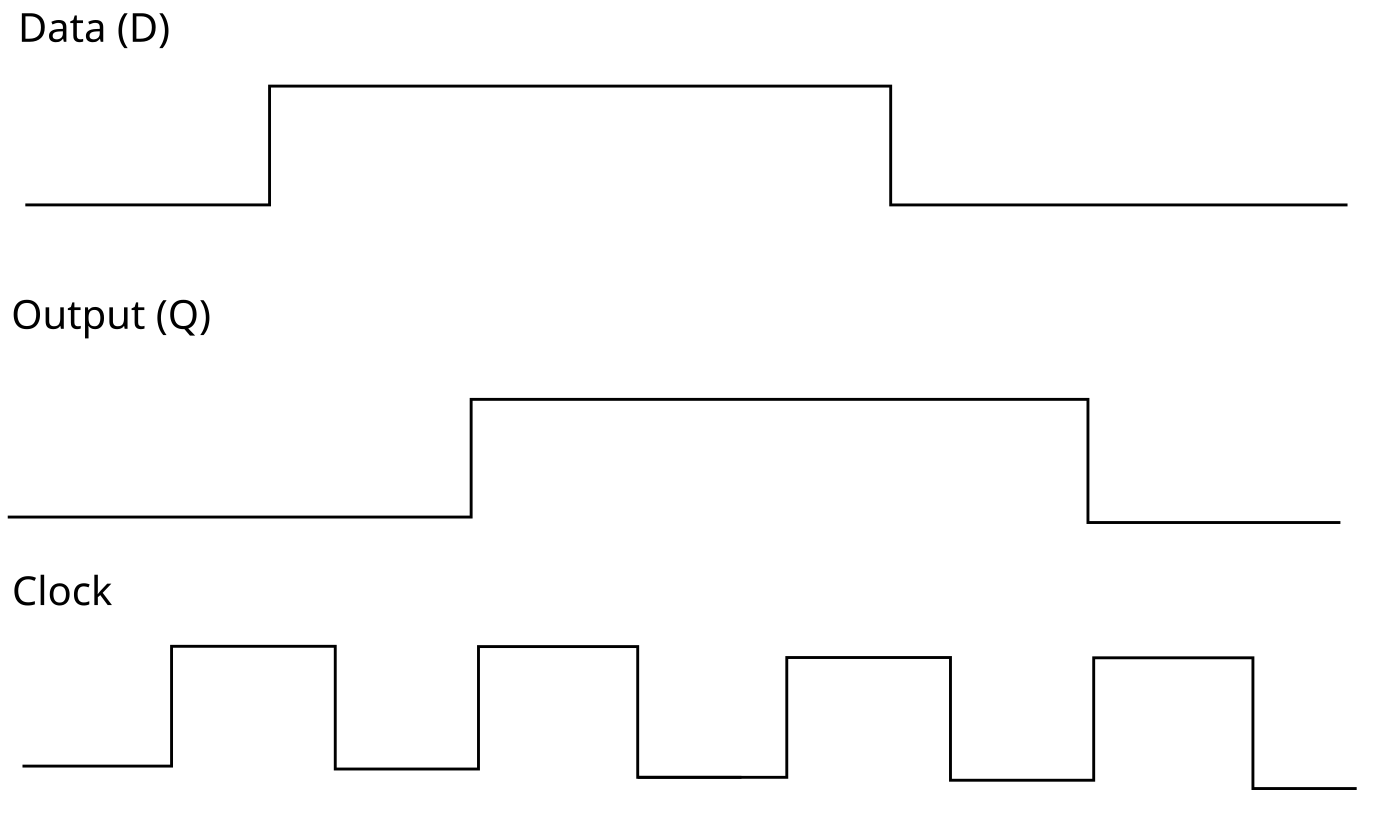
\includegraphics[scale=0.13]{flipflop_functionality.png}
        \caption{How a flip-flop reads output}
        \label{fig:flipflop_func}
    \end{subfigure}
\end{figure}

\subsection{Application specific integrated circuits}
As briefly explained in the introduction, if we after all this needed even more
speed we could implement this as an \textit{Application Specific Integrated
Circuit} (ASIC). Before we go into more detail, we'll give a brief overview
about logic gates. In Figure \ref{fig:logic_gate_explanation} we can see how
logic gates behave when different signals are sent through them. When we deal
with boolean functions addition is an OR gate, multiplication is an AND gate
and negation is a NOT gate. So if we go back to Example
\ref{ex:boolean_function} we can represent it using an OR and an AND gate as
seen in \ref{fig:logic_gate_impl}. We first calculate $B \cdot C$ after which
we send the result to the or gate and calculate $A + B \cdot C$. ASICs then use
this to implement all boolean functions, since they do not need to be able
to be reconfigured they can be made more efficient.

When making ASICs manufacturers often first create FPGA versions of them where
they create an FPGA with LUTs for each gate. Once they're tested thoroughly
they're made into ASICs.

\begin{figure}[H]
    \centering
    \begin{subfigure}[b]{.4\textwidth}
        \centering
        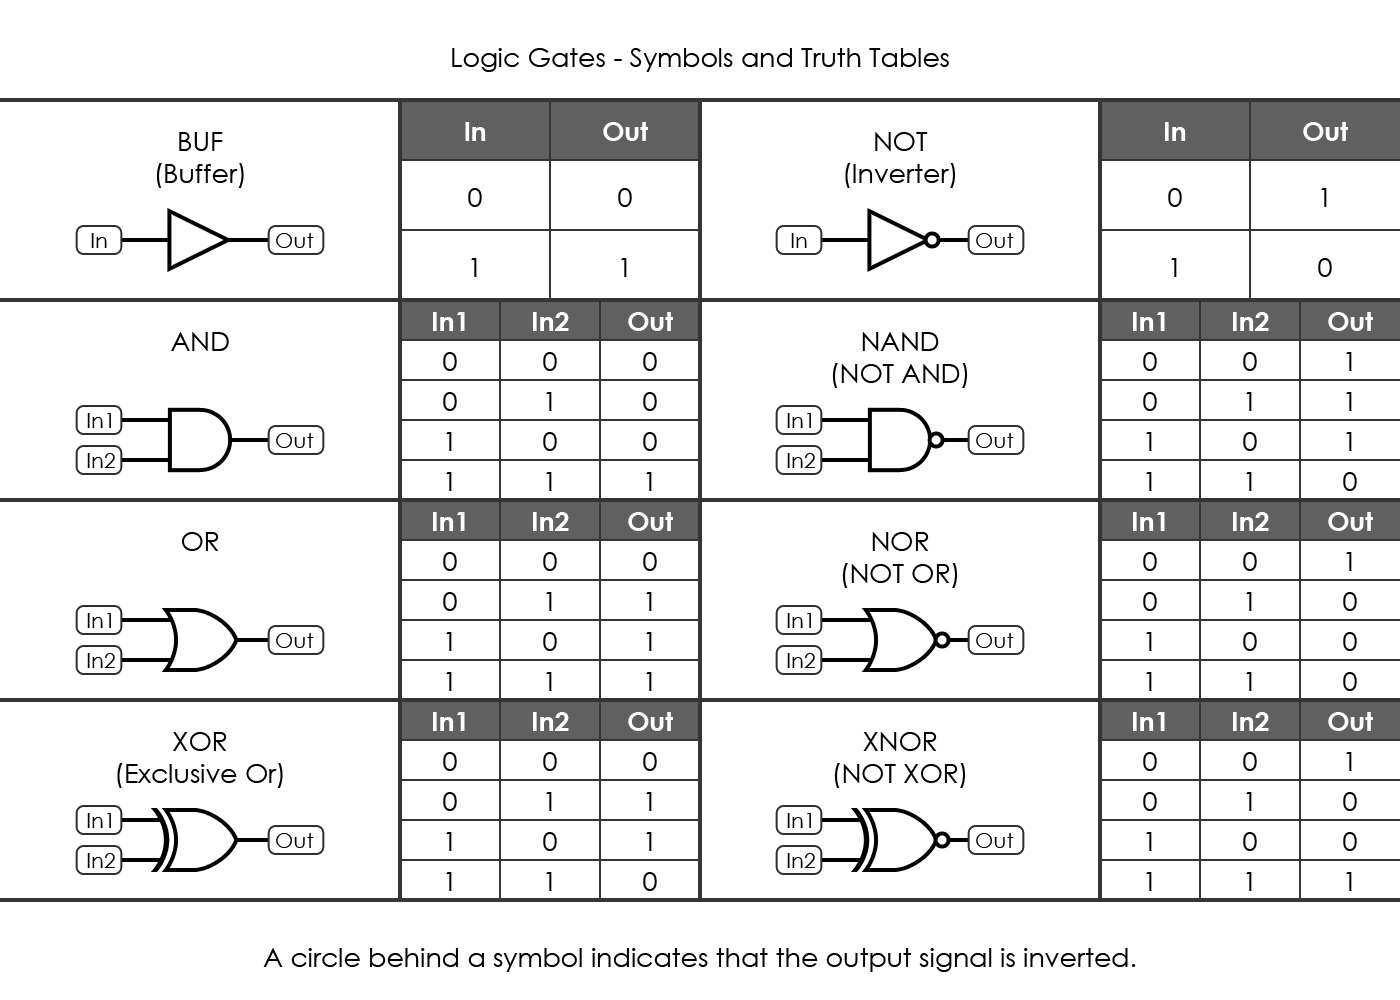
\includegraphics[scale=0.13]{logic_gate_explanation.jpg}
        \caption{An explanation of how different logic gates behave\citep{LogicGateBehavior}}
        \label{fig:logic_gate_explanation}
    \end{subfigure}
    ~
    \begin{subfigure}[b]{.4\textwidth}
        \centering
        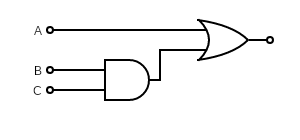
\includegraphics[scale=0.6]{circuit.png}
        \caption{Logic gate implementation of the function}
        \label{fig:logic_gate_impl}
    \end{subfigure}
\end{figure}

\begin{figure}[H]
    \centering
    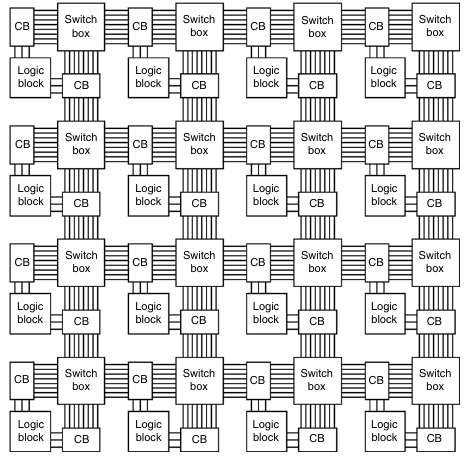
\includegraphics[scale=0.5]{fpga_structure.png}
    \caption{An example of an island-style FPGA\citep{M.MorrisMano3}}
    \label{fig:fpga_structure}
\end{figure}

\section{Input/Output blocks}
Input/Output blocks (I/O blocks, IOB) are blocks that are placed around the
periphery of the FPGA. They control the interface between the FPGA and external
circuits such as the clock and power usage.

\section{Connection block}
Along the wires by the logic blocks there are connection blocks (CB). These blocks
control which data goes into and out of a logic block. They also connect the
I/O blocks to the FPGA. In Figure \ref{fig:fpga_structure} we can see an
example of where these connection blocks could be placed.

\section{Switch block}
A switch block (switch box, SB) is a type of block that exists at every
intersection in the wiring. As the name suggests it is built from a bunch of
switches and it's job is to route the electricity between the logic blocks.
There are different types of implementations for switch blocks, depending on
the type it will have different levels of connectivity and efficiency. Though
the specifics of this is out of the scope of this paper.

\section{Connections}
There are multiple ways the logic blocks can be connected, for example Xilinx
FPGAs have four different types of interconnects: long lines, hex lines, double
lines and direct lines. The direct lines are to connect neighboring logic gates
for fast transfer. Hex and double lines connect logic gates that are a medium
length away. Long lines go along the entire chip and are often used for global
signals \citep{HideharuAmano8}.


\section{Configuration}
We will now give a brief overview on how these chips can be configured, though
we are only going to focus on the three main technologies: static RAM, flash
memory and antifuse. Depending on the technology used they can be more or less
configurable.

\subsection{Static RAM}
Static RAM, or SRAM is a very common way to handle configuration. It is great
because it is fast and has infinite reconfiguration. The issues with SRAM is
that it is volatile which means that if power is lost so is the configuration.
Another issue is power consumption, as the SRAM cell contains 6-12 transistors
compared to flash memory which only requires roughly two transistors
\citep{HideharuAmano8}.

\subsection{Flash memory}
Flash memory is a way to store the configuration in memory without needing
power for the chip to remember it. It works by having electrically erasable
programmable read-only memory, it's benefit is that the configuration can be
remembered even if the device is powered off. The downside is that there is only
a limited amount of writes before it fails and that flash is often slower at
writing than SRAM \citep{M.MorrisMano3}.

\subsection{Antifuse}
An antifuse is the opposite of a fuse, it works by having high resistance and
not allowing electricity to pass until the fuse is blown. This technology is
very reliable and rarely corrupts, which is why it is often used in places with
for example radiation \citep[Ch. 1]{ScottHauckAndreDeHon5}. The down side of antifuses is that it can only be
programmed once, after it's programmed the fuses are blown and can not be
restored.
